
\section{Game evaluation techniques}

\subsection{Introduction}


The computer game industry has been rapidly growing over the last few decades with revenues exceeding those made in the film industry in many areas~\citep{Mand06}. Despite this, the factors necessary for game success are not well understood. In addition, games are fundamentally different to many other forms of software as they serve the purpose of entertainment rather than aiding the user in attaining some goal~\citep{Swee05}. That is, when evaluating games one has to keep in mind issues, such as enjoyment and fun, which are not normally present in other types of software~\citep{Mand06}.

This introduces a number of other topics of investigation apart from just standard usability. It also highlights the need to draw on findings and research from other fields such as virtual reality and psychology~\citep{Swee05}. In particular, a focus on topics that allow one to assess enjoyment and emotional effect is needed. These topics include the fields of immersion, presence and flow which have previously been strongly linked to investigations of virtual environments and their related psychological correlates. This is not to say that traditional usability measures should be ignored, but rather that they should serve as a secondary, rather than primary, means for evaluating games~\citep{Hazl06}. However, with this said, it should be noted that conventional usability criteria need to be adapted to suit the gaming environment itself~\citep{Fede02}.

The current research in this field outlines a number of methods for collecting data on the playability and enjoyment produced by games. This includes surveys, questionnaires and interviews, heuristic methods, observational analysis as well as physiological means of evaluating player response. These methods range in both their quantitative and qualitative nature as well as how subjective or objective their means of data collection are~\citep{Mand06}. Figure~\ref{evalMethods} summarises the various available methods according to these criteria~\citep{Mand06}.
\begin{figure}
  \begin{center}
    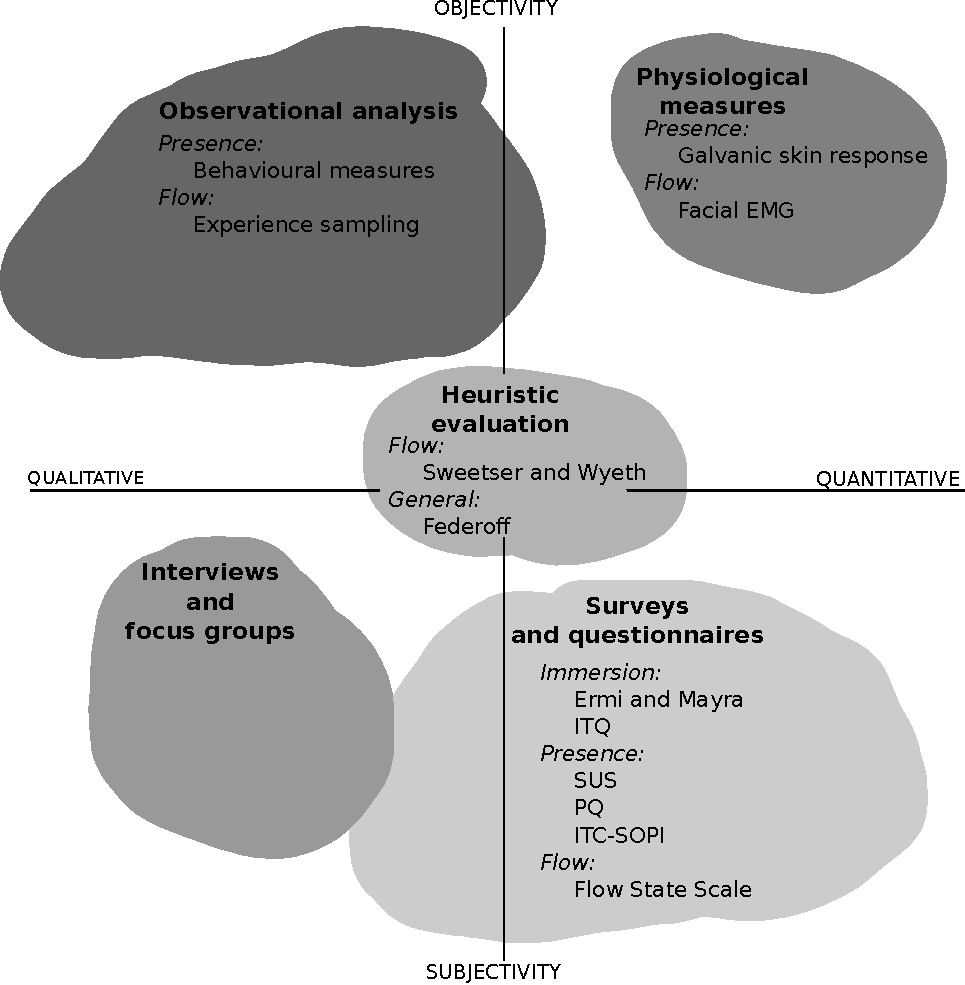
\includegraphics [scale=0.55]{drawing.pdf}

  \end{center}
  \caption{A summary of current research methods for games plotted according to how objective/subjective their data collection is as well as whether the data returned is qualitative or quantitative.}
  \label{evalMethods}
\end{figure}


This paper will provide a summary and comparison of these potential methodologies and how they can be applied to evaluating concepts such as immersion, presence and flow. In addition, ways of evaluating general usability issues will be considered. However, given that the single most important feature of any game is arguably the degree to which it provides enjoyment and entertainment for its players, this paper will focus more on how to measure and assess issues affecting this rather than on pure usability in the conventional sense.

\subsection{Computer games}
In order to better analyse the factors that lead to a game's success, one must first understand what differentiates games from other software. This is necessary as the metrics used to asses computer games must take into account these differences. The traditional concept of usability is defined as being composed of three independent measures: effectiveness, efficiency and satisfaction~\citep{Korh06}. However, within a game environment the first two measures appear to be far less important than the third~\citep{Fede02}.

This is perhaps because the most apparent difference is that games are generally designed purely to entertain users rather than assist them in completing some goal~\citep{Pine08}. In addition, individuals learn to play games without the use of manuals as well as developing their own techniques and strategies in order to increase their performance~\citep{Fede02}. Furthermore, whether or not a game succeeds at eliciting positive emotions is less dependant on the outcome and more on the actual process of playing~\citep{Mand06}. That is, unlike in other applications, players are unaware of what will happen next and often actively construct their potential experience~\citep{Korh06}. This is an important point as it means that much of the analysis should focus on how and whether a game elicits enjoyment and fun rather than just focusing on usability~\citep{Hazl06}. This also raises the question of how the process of game-play can be adequately assessed.

Finally, games do not provoke only positive emotions within players~\citep{Hazl06}. Rather, many games, through the use of challenges, appear to first develop negative emotions, such as frustration or forms of stress, which are then followed by positive emotions when the challenge is overcome~\citep{Ermi05}. Thus the affective aspect of games should also be considered as this may form a large part of what makes certain games more successful than others.

Overall, games differ significantly from non-leisure software applications as their primary goal is to entertain. This means that many existing techniques cannot be used in their current forms in order to assess computer games. Rather, an approach that attempts to integrate affective components with those of usability is needed to better gauge how and why users respond in particular ways to various games.

\subsection {Immersion}
One aspect that is thought to influence game enjoyment is immersion. This is defined by \citet{McMa06} as ``the objective level of fidelity of the sensory stimuli produced by a technological system". This can be further described as a psychological state mediated by an interface of sorts wherein the subject feels included in and constantly interacting with an environment through the means of a stream of experiences and stimuli~\citep{Witm98}.

The degree to which a user becomes immersed appears to lie along a continuum. That is, there are a number of preliminary stages a user proceeds through before reaching total immersion ~\citep{Brow04}. These initial states have been termed different things in the literature, from absorption~\citep{Ermi05} to engagement~\citep{Brow04} to involvement~\citep{Witm98}. However, all these terms appear to describe a state where attentional resources are directed towards an experience. This is distinct from full immersion as when a user becomes immersed they feel as if they are completely involved in a separate reality and thus direct all their attention and perceptual tools towards this environment~\citep{Ermi05}. There are thus parallels between full immersion and presence~\citep{Brow04}. However, it should be noted that full immersion is often very difficult to achieve~\citep{Witm98}.

This may be due to the fact that, in a sense, immersion requires the user to forget or overlook the fact that they are interacting with an environment through the means of some medium~\citep{Fede02}. This is often not possible in settings other than virtual reality. However, being able to gauge and measure immersion is of particular importance as immersion can be considered a necessary state in order for presence to be experienced~\citep{Brow04}. 

\subsubsection{Measuring immersion}
Assessing the degree of immersion has proved to be a difficult problem to solve~\citep{McMa06}. While there is much theoretical discussion of what immersion entails, there are very few methods of quantifying the level of immersion experienced by participants.

\citet{Ermi05} identified three aspects of immersion within the game-play experience. These are \textit{Sensory immersion}, which relates to the audiovisual environment of the game; \textit{Challenge-based immersion}, which refers to the match between a user's abilities and the challenge presented by the game, and \textit{Imaginative immersion}, which consists of the narrative dimension of the game experience. Using these three dimensions, a questionnaire was constructed to allow immersion to be assessed. However, while they did test their questionnaire on a number of different games, no statistical tests of \gls{intCon}, \gls{valid} or \gls{relia} were performed. Thus the validity of their findings and the usefulness of their survey remains questionable.

Another test of immersion, developed by \citet{Witm98}, measures the propensity an individual has to become immersed in an environment. The \gls{itq} uses three dimensions in order to do this. These are \textit{Involvement}, which assesses an individual's inclination to become passively immersed in some medium; \textit{Focus}, which refers to the degree a participant is able to concentrate on one task while blocking out other distractions, and \textit{Games}, which considers how often the individual plays games and how involved the individual becomes in the games when doing so~\citep{Witm98}. The test has been thoroughly evaluated to show it has a high internal consistency ($\alpha$ = 0.81) as well as displaying \gls{relia} and \gls{valid} (within each sub-scale)~\citep{Witm98}. 

While this questionnaire does not directly measure the amount of immersion experienced in a game environment, it is meant to provide an indication of how likely an individual is to experience presence~\citep{Witm98}. However, this correlation was not shown to be present in all tests conducted by the authors, despite an overall significant positive correlation (\emph{r} = 0.24, \emph{p} $<$ 0.01)~\citep{Witm98}.

Overall it appears that there are no concrete methods of evaluating the immersive effect of a game. This is potentially due to the very nature of immersion. However, as full immersion has been equated with presence, it may be more appropriate to attempt to quantify this construct instead~\citep{Brow04}.

\subsection{Presence}
Presence is defined as the ``perceptual illusion of nonmediation"~\citep{Rava04}. That is, a state where a user believes the environment presented through some medium is real~\citep{Ivor07}. Presence is of particular importance within a game environment as high levels are thought to increase the amount of enjoyment and fun experienced by players~\citep{Rava04}. Some research also suggests that presence has a positive influence on the ability to complete tasks~\citep{Ivor07}. While immersion and presence may appear to touch on a number of similar elements, they are in fact distinct concepts. Immersion is specifically concerned with the physical interface and its effects while presence refers to the psychological state produced by immersion and a myriad of other factors~\citep{Brow04}.

A number of different things that are thought to increase the possibility of presence have been identified in the literature. These can loosely be grouped into player and media characteristics~\citep{Less01}. Media characteristics refers to elements such as the narrative and overall story as well as the audiovisual and sensory characteristics of the game. For example, highly realistic and naturalistic displays and interaction techniques have been shown to positively contribute to the experience of presence~\citep{Less01}. 

Player characteristics include elements such as an individual's perceptual, motor and cognitive abilities as well as transient factors such as mood~\citep{Less01}. Furthermore, some research suggests that focus or selective attention, which refers to an individual directing their attention towards a particular stimuli while excluding others, can play an important role in eliciting and explaining presence~\citep{Witm98}. That is, with an increase in game difficulty, players are forced to expend more cognitive resources on interacting with the game and, by proxy, less attention is given to factors suggesting the game environment is not real~\citep{Rava04}. However, while this suggests that some form of attentional resource threshold exists in order for presence to be experienced, it is likely to be only one of many contributing factors~\citep{Witm98}.

Thus one needs to consider a variety of factors when assessing presence, both in terms of the simulated environment and in relation to the users themselves. 

\subsubsection{Measuring presence}
A number of methodologies have been used when attempting to measure presence. Due to the difficulty in both eliciting and measuring presence in situ, no well-accepted method has yet been developed~\citep{Mand06}. The following section will review the different techniques proposed in order to quantify presence.

A number of introspective techniques have been developed in order to assess presence. Perhaps the most widely used is the \gls{sus}~\citep{Blak10}. This questionnaire, administered after experiencing the game environment, consists of six items that require the participant to assess their level of presence~\citep{Ivor07}. While this scale has been shown to have \gls{faceVal}, it falls prey to many of the problems inherent in introspective measures. That is, due to its highly subjective nature, it suffers from issues of \gls{intCon} and \gls{valid}~\citep{Blak10}.

Introspection, however, does have its uses as a number of introspective, psychometrically validated studies exist. One of these, developed by \citet{Witm98}, consists of three sub-scales: \textit{Involved/Control}, which addresses issues of perceived control and responsiveness within the game; \textit{Natural}, which measures the extent to which the game was consistent with reality as well as how naturalistic elements such as interactions were, and \textit{Interface Quality}, which measures the extent to which participants were able to concentrate on tasks by examining whether control devices and displays distract or interfere with the task at hand~\citep{Witm98}. This presence scale is intended to be used in conjunction with the \gls{itq} mentioned above. Overall, the \gls{intCon} of this measure is high ($\alpha$ = 0.88), however, issues of \gls{consVal} remain suggesting the need for further research~\citep{Witm98}.

The Independent Television Commission's Sense of Presence Inventory [ITC-SOPI] is another introspective questionnaire~\citep{Blak10}. This attempts to quantify presence through the use of four independent sub-scales. These are \textit{Sense of Physical Space}, which refers to a feeling of being a part of the mediated environment; \textit{Engagement}, which includes emotional aspects related to fun and feeling psychologically involved with the environment; \textit{Ecological Validity}, which relates to believing elements in the environment were real, and \textit{Negative Effects}, which describes any adverse physiological effects that might lessen the sense of presence~\citep{Less01}. Cronbach's alpha was very high for all four scales, ranging between 0.77 and 0.94. In addition, the scales displayed sensitivity to cross-media comparisons as well as significant factor inter-correlations~\citep{Less01}. At present, the authors suggest that the four factors should be analysed separately in order to detect differences that may develop according to the type of media being assessed~\citep{Less01}. Overall, however, this scale provides a fairly reliable measure of presence~\citep{Blak10}.

Apart from introspective techniques, a number of behavioural and physiological methods also exist. Behavioural measures, however, are difficult to implement and may be subject to extraneous variables such as \gls{react}~\citep{Blak10}. Physiological assessment techniques rely on using involuntary physiological responses in order to gauge emotional responses. Some examples of these include monitoring heart rate or galvanic skin response. While some correlation has been shown between certain patterns of physiological response and results obtained using introspective presence questionnaires~\citep{Rava04}, there is still doubt as to whether certain physiological patterns can be unambiguously linked to presence~\citep{Blak10}. Furthermore, physiological measures often require expensive and specialised technology, meaning that they are not an appropriate measure for all circumstances~\citep{Blak10}.

Overall, while a number of different means for measuring presence exist, no one method has been shown to be superior to all others. With this said, however, the \gls{itc-sopi} appears to be the most reliable and psychometrically sound of the techniques discussed above. However, while the importance of assessing presence should not be overlooked, one must also consider other aspects of the game process, such as the ability to elicit enjoyment and fun from users.

\subsection{Flow}
Flow describes a game state where there is a successful balance between a player's ability and the perceived challenge or difficulty of the game~\citep{Ermi05}. However, what is important about this balance is the emotional reaction it produces within the player~\citep{John03}. \citet{Csik90} describes the experience of flow as being ``so gratifying that people are willing to do it for its own sake with little concern for what they will get out of it, even when it is difficult or dangerous". This description highlights the importance of attempting to create flow within a game environment.

Flow is thought to consist of eight interrelated elements. The first of these is a task that can be completed~\citep{Swee05}. The ability to concentrate on this task is also required. This concentration should be possible because the task has clear goals and/or because the task provides immediate feedback~\citep{John03}. The feeling of being able to exercise control over one's actions is also needed. All this leads to a deep involvement that removes awareness of everyday life, which in turn leads to one's concern for self disappearing~\citep{Swee05}. However, one's sense of self emerges stronger than before once the flow state is completed~\citep{Swee05}. Finally, the perceived duration of time is also altered during this state~\citep{John03}.

The application of flow to games would provide a powerful way of understanding the ways in which games manage to elicit enjoyment and fun despite, in general, serving no other intrinsic purpose.

\subsubsection{Measuring flow}
Flow is particularly difficult to measure as the only way to determine its presence during game-play is to disrupt it~\citep{Mand06}. That is, direct measures of flow end up disturbing the flow state itself. This problem has been tackled in a number of different ways which will be discussed below.

The first of these is to analyse a game according to a fixed set of heuristics that have been adapted to measure flow or potential elements that may disrupt flow. Such a set of heuristics, which draws upon the definition of flow as well as conventional usability standards, was developed by \citet{Swee05}. Their heuristics were found to have varying degrees of applicability depending on game genre~\citep{Swee05}. However, the applicability of heuristics to a topic such as enjoyment remains questionable. While heuristics are very useful for identifying potential problems in the game process, their use becomes less clear when attempting to understand the emotional effect of a scenario or environment on users~\citep{Mand06}.

Another method which may have some application to measuring flow is experience sampling. Experience sampling attempts to measure random instances of an individual's experience~\citep{Horm06}. In essence this method involves interrupting a user and then assessing whether one has in fact interrupted some sort of flow state~\citep{Mars05}. While this technique may seem counter-intuitive, it allows one to get glimpses into a user's current mental state~\citep{Horm06}. However, as this method relies on a participant's introspective analysis, it is subject to issues of \gls{relia}~\citep{Blak10}. 

The Flow State Scale, developed by \citet{Jack01}, is a questionnaire used to assess flow along the nine dimensions identified by~\citet{Csik90} as well as to provide an overall flow state score based on a higher order factor. The questionnaire comes in a number of variations that range in length, as well as the recommended time of administration (during the event versus after it)~\citep{Vlac00}. The long version of the scale has acceptable reliability ($\alpha$ = 0.83)~\citep{Jack01} and high internal consistency, with Cronbach's alpha equalling 0.93~\citep{Tene99}. A Rasch analysis conducted on the nine factors also suggests high consistency between and across samples~\citep{Tene99}. Finally, the questionnaire has also been shown to have acceptable discriminant and construct validity~\citep{Mars99}. Despite the high reliability and validity of this instrument, care should be taken in its use as it has primarily been evaluated in the context of sports and exercise-based activities~\citep{Jack01,Vlac00}.

A fourth technique is to use physiological methods in order to assess a player's emotional state. Through the use of techniques such as facial \gls{emg}, one is able to assess minute changes in facial expression and thus, by proxy, emotion~\citep{Hazl06}. Facial \gls{emg} thus allows the valence of a player's emotions to be measured~\citep{Mand06}. While there are other methods for measuring how positive or negative a player's emotions are, such as galvanic skin response and cardiovascular measures, facial \gls{emg} appears to be the most favoured by the research community and as such will be the only such measure discussed~\citep{Mand06}. 

The real benefit of such a technique is that it does not require interrupting game-play~\citep{Mand06}. In addition it allows for complex emotional profiles of game-play to be compiled. However, facial \gls{emg} is not without its caveats. To begin with, due to the sensitivity of the measure, it is easily influenced by external (and mentally internal) extraneous factors~\citep{Hazl06}. Furthermore, the need for special equipment means that cost may be a prohibiting factor~\citep{Blak10}. Finally, the use of such a method does not allow one to specifically identify which elements produce a favourable response, only that such a response is occurring~\citep{Hazl06}.

Overall, due to its nature, flow appears to be difficult to measure. While heuristics may prove useful they do not allow one to assess the actual flow process. Physiological measures, on the other hand, allow for this but may not identify specific aspects. Experience sampling allows for an intrusive combination of the two. The Flow State Scale seems to provide the best alternative, but is in need of further validation outside of a sports context. Which method is most appropriate may ultimately depend on the task being assessed and the resources available.


\subsection{General considerations}
In addition to research focusing specifically on issues such as immersion, presence and flow, much research has been done on general usability principles in games~\citep{Swee05}. The majority of these take the form of sets of heuristics that have been adapted from standard usability measures in order to assess games~\citep{Fede02}. These heuristics have proven to be of particular use in the design and development stages of a game~\citep{Desu04}. However, as mentioned above, a heuristic evaluation of elements other than usability and mechanics may prove difficult and unsatisfactory~\citep{Mand06}. Thus while heuristics should perhaps be considered in the design stages, they should be used only when appropriate~\citep{Swee05}.

\subsection{Conclusion}
Game enjoyment is a multifaceted issue which appears to depend on a large variety of determinants. These components, however, are interconnected and dependant. In addition to this, a shared difficulty in quantifying the degree to which each is elicited within a game environment appears to be a common factor.

Immersion, which describes a state where one feels one is a part of an environment, despite the technological system used to create said environment, appears to lack any concrete means of quantification. While means of doing so, such as the questionnaire developed by \citet{Ermi05}, do exist, the \gls{valid} of such instruments remains uncertain. Given the overlapping nature of full immersion in relation to presence, it may be more appropriate to measure presence instead. In addition, the use of the \gls{itq} questionnaire in conjunction with presence studies may provide valuable information on how dependant presence is on a person's innate immersive characteristics.

As mentioned, presence appears to be, at the very least, strongly dependant on an immersive state. Presence is defined as the perceptual illusion where an individual feels that an environment is real despite its virtual nature. While there is far more research on methods of evaluating presence in comparison to immersion, much of this research lacks a psychometrically sound basis. For this reason, should an in-depth study of the degree of presence elicited by a game be needed, the \gls{itc-sopi} questionnaire appears to be the most appropriate instrument. However, due to the short nature of other surveys, such as the \gls{sus} questionnaire, these surveys may be more useful when one wants to determine a more general level of presence in order to investigate something else.

Flow, which also appears to depend on immersion to some degree, can be thought of as a state where the intrinsic process of playing the game elicits enjoyment and euphoric feelings. Physiological measures, such as facial \gls{emg}, allow one to assess emotional valence during game-play thus avoiding interrupting the flow state. However, the need for special equipment may make such methods inappropriate. Experience sampling, despite its disruptive nature, allows for a simple means of determining whether the player subjectively felt they were experiencing flow. The Flow State Scale, on the other hand, provides a measure of flow without requiring the disruption of the current task. Due to the difficulty and cost associated with physiological measures and the disruptive nature of experience sampling, the Flow State Scale appears to be the most appropriate choice.

While heuristics do not appear to be relevant to measures of immersion, presence or flow, they should not be completely overlooked as they can serve a valuable purpose during the game development process. Since many such heuristics have been developed, a combination of a number of them may make for the most comprehensive coverage of the usability issues at hand.

Overall the topic of why people enjoy playing games is complex and multifaceted. However, since a fundamental component of the majority of games is to provide entertainment, this concept is of the utmost importance when evaluating games. Through the use of a variety of techniques, one can begin to assess the core issues at hand as well as to gain some insight into what may be done to improve the enjoyment experienced by players.



